\subsection{Backward projection methodology}
\label{spp:backward}

% This section has been modified and published at the ``Remote Sensing" \citep{wang_easyidp_2021}

\begin{center}
  \noindent
  \fbox{
    \begin{minipage}{0.95\textwidth}
    
      \begin{center}
        \textbf{EasyIDP: A Python Package for Intermediate Data Processing in UAV-Based Plant Phenotyping}
      \end{center}

      \noindent Haozhou Wang$^{1}$, Yulin Duan$^{2,3}$, Yun Shi$^{2,3}$, Yoichiro Kato$^{1,4}$, Seishi Ninomiya$^{1,5}$, and Wei Guo$^{1,\star}$
    
      \noindent $^{1}$ International Field Phenomics Research Laboratory, Institute for Sustainable Agro-Ecosystem Services, Graduate School of Agricultural and Life Science, The University of Tokyo, Tokyo 188-0002, Japan;
      
      \noindent $^{2}$ Key Laboratory of Agricultural Remote Sensing, Ministry of Agriculture, Beijing 100081, China;

      \noindent $^{3}$ Institute of Agricultural Resources and Regional Planning, Chinese Academy of Agricultural Sciences, Beijing 100081, China

      \noindent $^{4}$ International Rice Research Institute, Metro Manila 1226, Philippines

      \noindent $^{5}$ Plant Phenomics Research Center, Jiangsu Collaborative Innovation Center for Modern Crop Production, Nanjing Agricultural University, Nanjing 210095, China
      
      \noindent $^{\star}$ Corresponding author

      \begin{spacing}{1.5}
      \textbf{Abstract}
      \end{spacing}
      
      Unmanned aerial vehicle (UAV) and structure from motion (SfM) photogrammetry techniques are widely used for field-based, high-throughput plant phenotyping nowadays, but some of the intermediate processes throughout the workflow remain manual. For example, geographic information system (GIS) software is used to manually assess the 2D/3D field reconstruction quality and cropping region of interests (ROIs) from the whole field. In addition, extracting phenotypic traits from raw UAV images is more competitive than directly from the digital orthomosaic (DOM). Currently, no easy-to-use tools are available to implement previous tasks for commonly used commercial SfM software, such as Pix4D and Agisoft Metashape. Hence, an open source software package called easy intermediate data processor (EasyIDP; MIT license) was developed to decrease the workload in intermediate data processing mentioned above. The functions of the proposed package include (1) an ROI cropping module, assisting in reconstruction quality assessment and cropping ROIs from the whole field, and (2) an ROI reversing module, projecting ROIs to relative raw images. The result showed that both cropping and reversing modules work as expected. Moreover, the effects of ROI height selection and reversed ROI position on raw images to reverse calculation were discussed. This tool shows great potential for decreasing workload in data annotation for machine learning applications.

      \vspace{5mm}
      \textbf{keywords}: orthomosaic; photogrammetry; phenotyping; reverse calculation; Pix4D; Agisoft Metashape; Agisoft PhotoScan

    \end{minipage}
  }
\end{center}

The function of this backward projection is projecting ROI from world coordinate to relative UAV raw images. In this section, using ``zipfile" and ``xml" Python packages to load the external and internal camera parameters generated from SfM-MVS reconstruction projects. Then apply the backward calculation using the pinhole camera model. Finally camera distortion calibration is conducted.

\subsubsection{Camera parameters loading}

The relationship between field and UAV raw images is built after running SfM-MVS software. It has two main parts, external and internal parameters. The external parameters are different for each raw image, including the camera position (x, y, z) in the real-world coordinate ($O_{world}$, Fig.~\ref{fig:idps1}.a) and the camera rotation (yaw, pitch, roll). The internal parameters describe the characteristics of the sensor and are the same as each raw image, such as focal length, camera Charge-coupled Device (CCD) size, and lens distortion calibration parameters (\url{https://support.pix4d.com/hc/en-us/articles/202559089-How-are-the-Internal-and-External-Camera-Parameters-defined}). These parameters are available under the Agisfot Metashape and Pix4D project intermediate files.

For Pix4D projects, all these parameters are located in the ``1\_initial/params" folder, the ``calibrated internal camera parameters.cam", ``calibrated camera paramters.txt", ``pmatrix.txt", and ``offset.xyz" are loaded as text directly and parsed in the EasyIDP package without any external packages. For more details about those files, please refer to the Pix4D official documentation (\url{https://support.pix4d.com/hc/en-us/articles/202559089-How-are-the-Internal-and-External-Camera-Parameters-defined}).

For Agisoft Metashape projects, all these parameters can be obtained either by calling APIs (Professional license required) or by reading zipped xml files in the project file ``project.files/0/chunks.zip/doc.xml". The EasyIDP package chose the zipped xml way without a professional license. The ``zipfile" and ``xml" packages were used to un-zip and parse these parameters in xml files.

\begin{figure}[htb]
  \begin{center}
    \resizebox{\textwidth}{!}{
      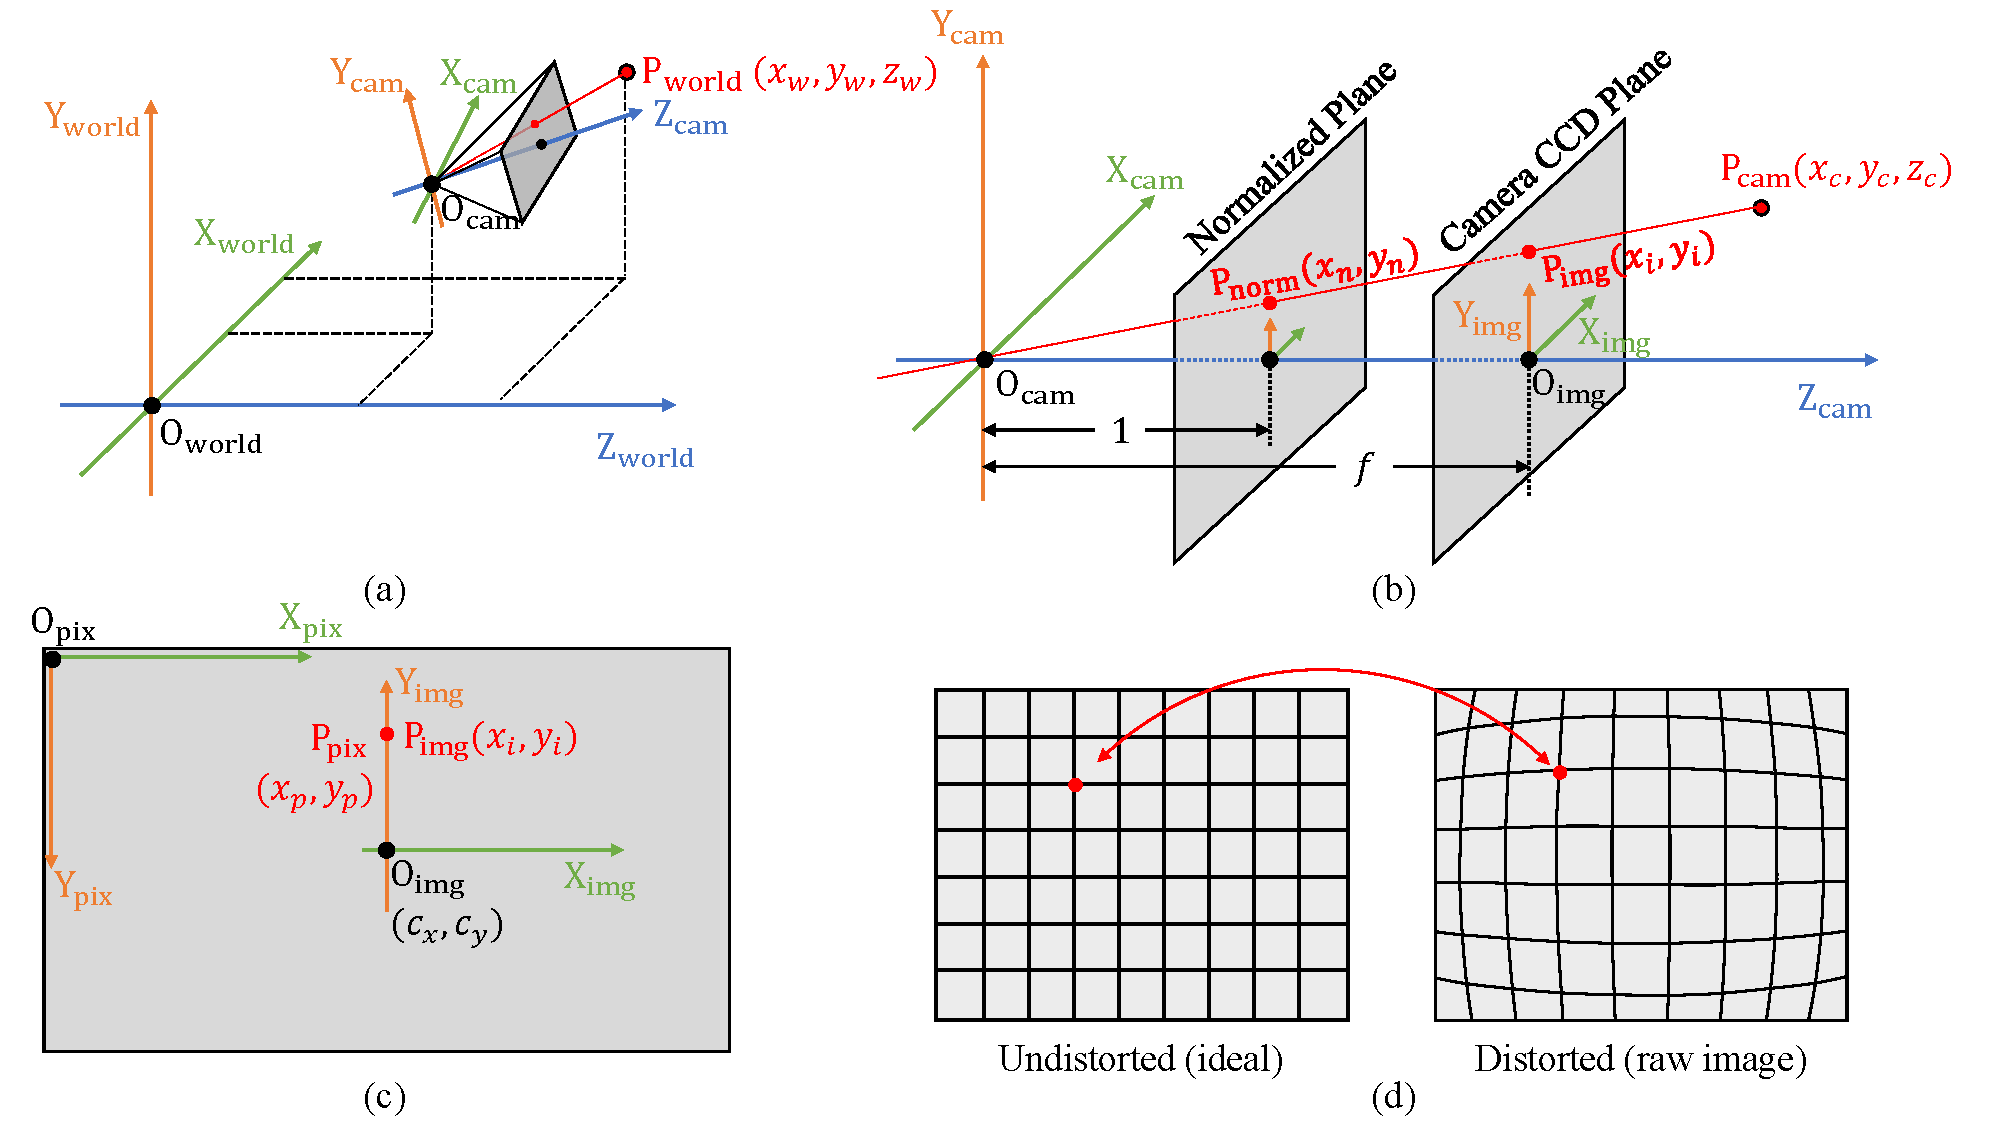
\includegraphics{figures/idp/Fig.S1_world2pixels.pdf}
    }
  \end{center}
  \caption[Backard projection illustration graph]{
     Backard projecting one point from the 3D world coordinates to the 2D pixel coordinates on raw UAV images by pinhole camera model. (a) The relationship between world coordinate ($O_{world}$) and camera coordinate ($O_{cam}$), linked by camera external parameters (position and rotation). (b) the relationship between camera coordinate ($O_{cam}$) and image coordinate ($O_[img]$). (c) The relationship between image coordinate ($O_[img]$) and pixel coordinate ($O_{pix}$). (d) The camera distortion calibration between undistorted images and distorted images caused by the lens.
  }
  \label{fig:idps1}
\end{figure}

\subsubsection{Backward projection formulas}

The geometry from the real-world coordinate ($O_{world}$) to image pixel coordinate ($O_{pix}$) is shown in Fig. \ref{fig:idps1}.a-c. There are four coordinate systems, first is the $O_{world}$ whose unit is often meter (Fig. \ref{fig:idps1}.a). The second one is the camera coordinate ($O_{cam}$, Fig. \ref{fig:idps1}.b), which makes the camera position to the origin (0,0,0) of coordinates, and the camera optical axis is used as the z-axis (commonly, the point $O_{img}$ is not the center point of plane). The third is the camera CCD coordinate ($O_{img}$, Fig.~\ref{fig:idps1}.c) whose unit is often mm. The last one is pixel coordinate ($O_{pix}$) whose origin is the top left corner in the $O_{img}$ and the unit is pixel.

Let us assume a point $P_{world} (x_w,y_w,z_w)$ in $O_{world}$, to transform that point into $P_{cam} (x_c,y_c,z_c)$ in $O_{cam}$ (Fig.~\ref{fig:idps1}.a), the $3\times4$ transform matrix $T$ could be derived from camera position ($t$, translational transformation) and camera rotation ($R$, rotational transformation):

\begin{equation}
  \begin{array}{lll}
    P_{cam} & = & T \cdot P_{world} \\
    \begin{small}
      \left[ 
        % amsmath package is required
        \begin{matrix} 
          x_c \\
          y_c \\
          z_c \\
        \end{matrix} 
      \right] 
    \end{small}
    & = & 
      \begin{small}
      \left[ 
        % amsmath package is required
        \begin{matrix} 
          R_{11} & R_{12} & R_{13} & t_1 \\
          R_{11} & R_{12} & R_{13} & t_1  \\
          R_{11} & R_{12} & R_{13} & t_1  \\
        \end{matrix} 
      \right] 
      \left[ 
        % amsmath package is required
        \begin{matrix} 
          x_w \\
          y_w \\
          z_w \\
          1
        \end{matrix} 
      \right] 
    \end{small}
  \end{array}
\label{eq:idp1}
\end{equation}

\noindent 
Where, $t$ is the $3\times1$ position matrix, and $R$ is the $3\times3$ rotation matrix derived by $(\omega, \varphi, \kappa)$ from camera rotation parameters (yaw, pitch, roll) (\url{https://support.pix4d.com/hc/en-us/articles/202558969-Yaw-Pitch-Roll-and-Omega-Phi-Kappa-angles}):

% \begin{equation}
  \begin{array}{lll}
    R & = & R(\omega) R(\varphi) R(\kappa) \\
    & = &
      \begin{small}
      \left[ 
        % amsmath package is required
        \begin{matrix} 
          1 & 0           & 0 \\
          0 & cos(\omega) & -sin(\omega) \\
          0 & sin(\omega) & cos(\omega)
        \end{matrix} 
      \right] 
      \left[ 
        \begin{matrix} 
          cos(\varphi)  & 0 & sin(\varphi) \\
          0             & 1 & 0 \\
          -sin(\varphi) & 0 & cos(\varphi)
        \end{matrix} 
      \right] 
      \left[ 
        \begin{matrix} 
          cos(\kappa) & -sin(\kappa) & 0 \\
          sin(\kappa) & cos(\kappa)  & 0 \\
          0           & 0            & 1
        \end{matrix} 
      \right] 
      \end{small} \\ \\
    & = &
      \begin{small}
        \left[ 
          \begin{matrix} 
            cos \kappa cos \varphi  
              & -sin \kappa cos \varphi  
              & sin \varphi  \\
        
            cos \kappa sin \omega sin \varphi  + sin \kappa cos \omega 
              & cos \kappa cos \omega  - sin \kappa sin \omega sin \varphi 
              & -sin \omega cos \varphi  \\
        
            sin \kappa sin \omega  - cos \kappa cos \omega sin \varphi 
              & sin \kappa cos \omega sin \varphi  + cos \kappa sin \omega  
              & cos \omega cos \varphi 
          \end{matrix} 
        \right] 
      \end{small} \\ \\
    & = &
      \begin{bmatrix}
        R_{11} & R_{12} & R_{13} \\
        R_{11} & R_{12} & R_{13} \\
        R_{11} & R_{12} & R_{13} \\
      \end{bmatrix}
  \end{array}
  \label{eq:idp2}
\end{equation}

The distance from the normalized plane to the origin $O_{cam}$  is 1 mm while the distance from the camera CCD plane to the origin $O_{cam}$ is focal length $f$ (Fig.~\ref{fig:idps1}.b) in mm. The transformation from $P_{cam}(x_c,y_c,z_c)$ to normalized plane $P_{norm} (x_n,y_n)$ and camera CCD plane $P_{img} (x_i,y_i)$ can be derived by triangle similarity:

\begin{equation}
  \begin{bmatrix} 
    x_i \\ y_i \\ 1
  \end{bmatrix} 
  = f
    \begin{bmatrix} 
      x_n \\ y_n \\ 1
    \end{bmatrix} 
  = f
    \begin{bmatrix} 
      \frac{x_c}{z_c} \\
      \frac{y_c}{z_c} \\
      1
    \end{bmatrix} 
  = \frac{f}{z_c}
    \begin{bmatrix} 
      x_c \\ y_c \\ z_c
    \end{bmatrix} 
\label{eq:idp3}
\end{equation}

To transform $P_{img} (x_i,y_i)$ in mm to the image pixel coordinate position $P_{pix} (x_p,y_p)$ in pixel (Fig.~\ref{fig:idps1}.c), the following set of equations should be applied:

\begin{equation}
  \left\{
  \begin{array}{lllllll}
    x_p & = & \alpha \cdot x_i + c_x 
        & = & f \cdot \alpha \cdot x_n + c_x 
        & = & f_{\alpha} \cdot x_n + c_x \\
    y_p & = & \beta \cdot y_i + c_y 
        & = & f \cdot \beta \cdot y_n + c_y 
        & = & f_{\beta} \cdot y_x + c_y
  \end{array}
  \right.
\label{eq:idp4}
\end{equation}

\noindent 
Where, $\alpha$ and $\beta$ are the pixel resolution whose unit is pixel/mm, and often are the same in pinhole camera models. $f_{\alpha}$ and $f_{\beta}$ is the focal length in pixel. Notably, Pix4D $(c_x,c_y)$ can be obtained directly, while for Agisoft Metashape (\url{https://www.agisoft.com/pdf/metashape-pro_1_7_en.pdf.} p. 176), $(c_x,c_y)$ in the xml file is not what is defined here, it is the offset to image center, which actually equals to $(0.5w+c_x,0.5h+c_y)$, where $w$ and $h$ are the pixel width and pixel height, respectively.

Equations \eqref{eq:idp4} can be expressed in the following homogeneous coordinate form: 

\begin{equation}
  \begin{bmatrix}
    x_p \\ y_p \\ 1 
  \end{bmatrix}
  =
  \begin{bmatrix}
    f_{\alpha} & 0         & c_x \\
    0          & f_{\beta} & c_y \\
    0          & 0         & 1
  \end{bmatrix}
  \begin{bmatrix}
    x_n \\ y_n \\ 1
  \end{bmatrix}
  = K
  \begin{bmatrix}
    x_n \\ y_n \\ 1
  \end{bmatrix}
\label{eq:idp5}
\end{equation}

Sum up equations \eqref{eq:idp1} to \eqref{eq:idp5}; to transform $P_w (x_w,y_w,z_w)$ directly to $P_{pix} (x_p,y_p)$:

\begin{equation}
  \begin{bmatrix}
    x_p \\ y_p \\ 1 
  \end{bmatrix}
  = K
    \begin{bmatrix}
      x_n \\ y_n \\ 1
    \end{bmatrix}
  = \frac{1}{z_c} K 
    \begin{bmatrix}
      x_c \\ y_c \\ 1
    \end{bmatrix}
  = \frac{1}{z_c} 
    \begin{bmatrix}
      K & 1
    \end{bmatrix}
    T
    \begin{bmatrix}
      x_w \\ y_w \\ z_w \\ 1
    \end{bmatrix}
  = P_{mat}
    \begin{bmatrix}
      x_w \\ y_w \\ z_w \\ 1
    \end{bmatrix}
\label{eq:idp6}
\end{equation}

\noindent
where the $3\times4$ matrix $P_{mat}$ is often called the projection matrix, which can directly transform points in 3D world coordinates to 2D pixel coordinates.

\subsubsection{Camera distortion calibration}

The equation \eqref{eq:idp5} transformation is idealized, and the distortion caused by the camera lens is neglected (Fig.~\ref{fig:idps1}.d). Several camera calibration parameters are used to correct this distortion, including three or four radial distortion coefficients ($K_i$ in MetaShape and $R_i$ in Pix4D) and two tangential distortion coefficients ($P_i$ in MetaShape and $T_i$ in Pix4D). Metashape sometimes provides affinity ($B_1$) and non-orthogonality ($B_2$) coefficients in pixels. The correction equation to distorted pixel position $(x_p^\prime,y_p^\prime)$ are as follows:

\begin{equation}
  \begin{array}{lll}
  \text{Pix4D} & = &
    \begin{cases}
      x_p^\prime =  c_x + x^\prime f \\
      y_p^\prime =  c_y + y^\prime f 
    \end{cases}
  
  \\ \\

  \text{Metashape} & = &
    \begin{cases}
      x_p^\prime = c_x + x^\prime f + x^\prime B_1 + y^\prime B_2 \\
      y_p^\prime = c_y + y^\prime f 
    \end{cases}

  \end{array}
\label{eq:idp7}
\end{equation}

\noindent
where:

\begin{equation}
  \begin{array}{lll}
    \text{Pix4D} & = &
    \begin{cases}
      x^\prime = k_0 x_n + 2 T_2 x_n y_n + T_1(r^2 + 2 x_n^2) \\
      y^\prime = k_0 y_n + 2 T_1 x_n y_n + T_2(r^2 + 2 y_n^2)
    \end{cases}
  
  \\ \\

  \text{Metashape} & = &
    \begin{cases}
      x^\prime = k_0 x_n + 2 P_2 x_n y_n + P_1(r^2 + 2 x_n^2) \\
      y^\prime = k_0 y_n + 2 P_1 x_n y_n + P_2(r^2 + 2 y_n^2)
    \end{cases}
  \end{array}
\label{eq:idp8}
\end{equation}

\noindent
and: 

\begin{equation}
  \begin{array}{llll}
    r   & = & \sqrt{x_n^2 + y_n^2} & \\ \\
    k_0 & = & 
      \begin{cases}
        1 + R_1 r^2 + R_2 r^4 + R_3 r^6           & (\text{Pix4D}) \\
        1 + K_1 r^2 + K_2 r^4 + K_3 r^6 + K_4 r^8 & (\text{Metashape})\\
      \end{cases}
  \end{array}
\label{eq:idp9}
\end{equation}